\section{Précision de la verrerie}

Voici deux instruments de mesure :

\begin{center}
	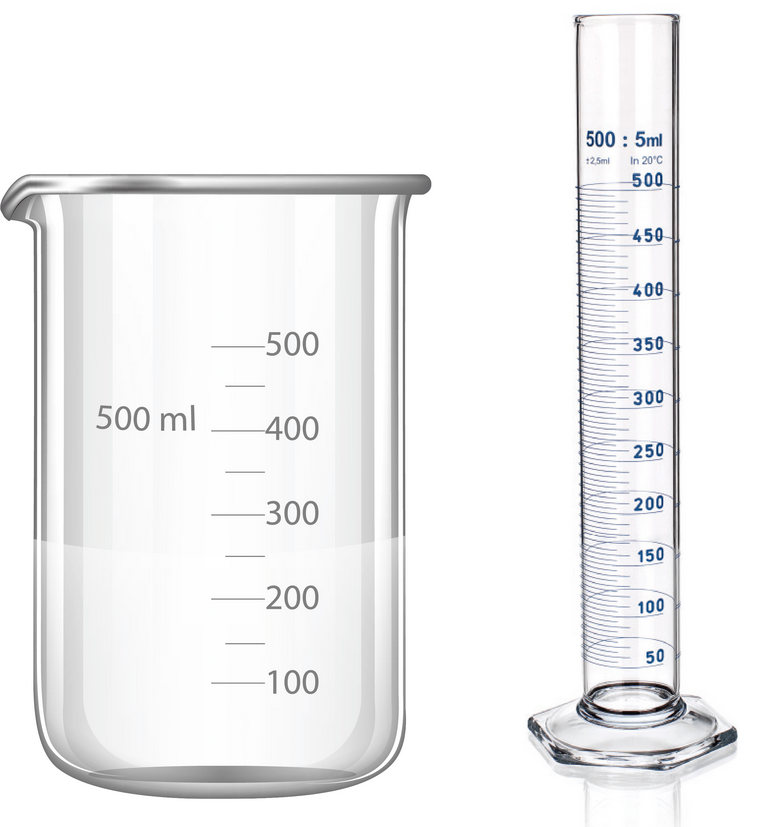
\includegraphics[scale=0.3]{img/vol}
\end{center}

\begin{questions}
	\question[] Quel est leur nom ?

		\begin{solution}
			
		\end{solution}
	
	\question[] Quelle est l'unité de mesure utilisée pour ces instruments de mesure ?

	\question[] Dans chaque cas, à quel volume correspond un intervalle ?
	
	\question[] Si l'on se trompe d'une graduation, quelle sera l'erreur commise sur la mesure ?
	
	\question[] Lequel de ces instruments permet d'effectuer la masure la plus précise ?
	
	\question Existe-t-il une relation entre le diamètre de l'instrument de mesure et la précision des mesures ?

\end{questions}